% main.tex — Informe Final: Dólar Blue Bolivia (CRISP-DM)
% Compilar: make render  (o: tectonic -o build main.tex desde report/)
\documentclass[11pt,a4paper]{article}

% ------------------------- Idioma y tipografía -------------------------
\usepackage[spanish,es-tabla,es-noshorthands]{babel}
\usepackage{fontspec}            % motor XeTeX (tectonic): UTF-8 nativo
\usepackage[htt]{hyphenat}       % permite cortar líneas dentro de \texttt{}

% ------------------------- Matemáticas y tablas -------------------------
\usepackage{amsmath}
\usepackage{booktabs}
\usepackage{multirow}

% ------------------------- Gráficos y color -------------------------
\usepackage{graphicx}
\graphicspath{{figures/}}
\usepackage{xcolor}
\definecolor{dbblue}{HTML}{2563EB}   % paleta del proyecto (eda_report.py)
\definecolor{dborange}{HTML}{F59E0B}
\definecolor{dbgray}{HTML}{6B7280}

% ------------------------- Números en español -------------------------
\usepackage{siunitx}            % coma decimal: \num{12,5}
\sisetup{output-decimal-marker={,}}

% ------------------------- Página y flotantes -------------------------
\usepackage[a4paper,margin=2.5cm]{geometry}
\usepackage[font=small,labelfont=bf]{caption}
\usepackage{float}
\usepackage[section]{placeins}  % las figuras no cruzan de subsección
\emergencystretch=1.5em  % evita overfull por tokens \texttt{} largos

% ------------------------- Enlaces -------------------------
\usepackage[colorlinks=true,linkcolor=dbblue,urlcolor=dbblue,citecolor=dbblue]{hyperref}

% ------------------------- Bibliografía -------------------------
% natbib + BibTeX clásico: tectonic lo ejecuta internamente (sin biber).
\usepackage[numbers,sort&compress]{natbib}
\bibliographystyle{plainnat}
\addto\captionsspanish{\renewcommand{\refname}{Bibliografía}}

% ------------------------- Título -------------------------
\title{Relación entre el tipo de cambio oficial (BCB), el mercado
       paralelo (dólar blue) y el mercado P2P (USDT) en Bolivia\\[0.5em]
       \large Informe final --- Proyecto de Data Science (CRISP-DM)}
\author{Franz Eulate}
\date{\today}

\begin{document}

\maketitle

\begin{abstract}
\noindent
Bolivia opera con dos sistemas de precios del dólar: el tipo de cambio
oficial administrado por el BCB y el mercado paralelo (\emph{dólar blue})
que se forma en plataformas P2P de criptomonedas. Este informe documenta,
siguiendo la metodología CRISP-DM \cite{chapman2000crisp},
las fases de comprensión del negocio, comprensión de los datos, preparación
y modelado, cuyo objetivo es \textbf{predecir} el nivel del paralelo y la
brecha oficial--paralelo a horizontes de una hora y un día. Se describe el pipeline
que recolecta y normaliza las cotizaciones de la API pública de
dolarbluebolivia.click y de la Gaceta Oficial de Bolivia, el análisis
exploratorio de la brecha, la tabla de características y los modelos de
previsión (regresión lineal, OLS con errores HAC y ARIMA) evaluados contra
una línea base naïve en una ventana de prueba de las últimas 168~h (una semana), con
frecuencia horaria.

\medskip
\noindent\textit{Datos al: 2026-10-24 02:33 UTC
\unskip.}

\end{abstract}

\section*{Introducción}
\label{sec:introduccion}

\subsection{Motivación}

Desde 2023 Bolivia atraviesa una escasez de divisas que separó de forma
persistente el tipo de cambio oficial, administrado por el Banco Central de
Bolivia (BCB), del precio que el dólar alcanza en el mercado paralelo
(\emph{dólar blue}). Tras el régimen flexible de 2025--2026, el oficial quedó
unificado mientras el paralelo cotiza libremente vía USDT en plataformas P2P
(Binance, Bybit, Bitget) y fintechs (Airtm, Takenos, El Dorado,
Wallbit). Esa \textbf{brecha} es el
principal termómetro de escasez de divisas y de presión cambiaria del país.

\subsection{Alcance}

Este informe documenta, siguiendo la metodología CRISP-DM
\cite{chapman2000crisp}, la construcción de un pipeline de
datos reproducible que:

\begin{itemize}
  \item recolecta y normaliza cotizaciones de la API pública de
        \href{https://www.dolarbluebolivia.click}{dolarbluebolivia.click}
        (37 endpoints) \cite{dolarblue2026api} y de la Gaceta Oficial de
        Bolivia \cite{gaceta2026};
  \item mantiene series de tiempo alineadas blue/oficial (compra/venta);
  \item produce análisis exploratorio reproducible;
  \item ajusta modelos de \textbf{previsión} del nivel del paralelo y de la
        brecha oficial--paralelo (regresión lineal, OLS con errores HAC y
        ARIMA), evaluados con partición temporal y línea base naïve a un
        horizonte de 1~hora y 1~día (Objetivo 1), y estudia la \textbf{relación}
        entre las publicaciones de la Gaceta y la brecha en horizontes de
        horas a días (Objetivo 2);
\end{itemize}

\subsection{Estructura del documento}

La \hyperref[sec:negocio]{sección~\ref*{sec:negocio}} desarrolla la comprensión
del negocio (problema de predicción, Objetivos 1--2, criterios de éxito,
recursos disponibles). La
\hyperref[sec:datos]{sección~\ref*{sec:datos}} describe las fuentes, el
pipeline de recolección y el diccionario de datos. La
\hyperref[sec:analisis]{sección~\ref*{sec:analisis}} presenta el análisis
exploratorio y la \hyperref[sec:preparacion]{sección~\ref*{sec:preparacion}}
la preparación de datos (fase 3) y la
\hyperref[sec:modelado]{sección~\ref*{sec:modelado}} reporta el modelado
(fase 4). La \hyperref[sec:negocio_eval]{sección~\ref*{sec:negocio_eval}}
traduce las métricas a KPIs de negocio y ROI (fase 5). El despliegue y el
monitoreo (fase 6) quedan como trabajo pendiente.

\section{Comprensión del negocio}
\label{sec:negocio}

Proyecto: relación entre el tipo de cambio oficial (BCB), el mercado paralelo
(\emph{dólar blue}) y el mercado P2P de USDT en Bolivia.

\subsection{Objetivo del negocio y KPIs}

\subsubsection{Definición del problema}

En Bolivia conviven \textbf{dos sistemas de precios del dólar} que no siempre
coinciden:

\begin{itemize}
  \item el \textbf{tipo de cambio oficial}, administrado por el Banco Central de
        Bolivia (BCB), que rige para operaciones bancarias formales, y
  \item el \textbf{mercado paralelo o ``dólar blue''}, que se forma libremente en
        plataformas P2P de criptomonedas (Binance, Bybit, Bitget) y
        fintechs (Airtm, Takenos, El Dorado, Wallbit), cotizado en USDT.
\end{itemize}

La \textbf{brecha} entre ambos es el principal termómetro de escasez de divisas
y de presión cambiaria. El problema que aborda este proyecto es de
\textbf{previsión}: los actores del mercado (importadores, empresas y personas)
no pueden anticipar el nivel futuro del paralelo, y por lo tanto no pueden
planificar tesorería ni cobertura con antelación. Se identifican dos problemas
específicos:

\begin{enumerate}
  \item \textbf{Falta de anticipación} --- no existen estimaciones del nivel del
        paralelo ni de la brecha a horizontes cortos (1~hora y 1~día). Predecir el
        tipo de cambio fuera de muestra es un problema reconocidamente difícil,
        en el que los modelos estructurales suelen no superar al paseo aleatorio
        ; aun así, enfoques de aprendizaje automático
        han mostrado capacidad predictiva en mercados financieros.
  \item \textbf{Relación no cuantificada} --- se desconoce si las normas
        publicadas en la Gaceta Oficial (combustibles, controles de cambio,
        reservas, deuda, etc.) anticipan o acompañan movimientos de la brecha;
        sin esa evidencia no pueden usarse como señales de política.
\end{enumerate}

Adicionalmente, la información está fragmentada entre fuentes heterogéneas
(BCB, bancos, agregadores y plataformas P2P), lo que condiciona la recolección
de datos y la construcción de una serie única de trabajo.

Definir con precisión este problema determina \textbf{qué datos recolectar}
(series de precios por fuente con marca de tiempo y origen, volúmenes) y
\textbf{cómo interpretar los análisis} (toda métrica se lee
como distancia frente al precio oficial administrado, no como precio absoluto),
y fija el criterio de éxito: la capacidad de \textbf{anticipar} el paralelo y
la brecha, y de vincular sus movimientos con las publicaciones de política.

\subsubsection{Objetivos}

\begin{table}[!ht]
\centering\small
\begin{tabular}{@{}p{0.15\textwidth}p{0.75\textwidth}@{}}
\toprule
\# & Objetivo \\
\midrule
Objetivo 1 & Predecir el nivel del paralelo y la brecha oficial--paralelo a
      1~h y 1~día, con intervalos de predicción \\
Objetivo 2 & Cuantificar la relación entre las publicaciones de la Gaceta
      (canales temáticos) y la brecha, en ventanas de $\pm5$ días \\
\bottomrule
\end{tabular}
\caption{Objetivos de predicción.}
\label{tab:objetivos}
\end{table}

\subsection{Criterios de éxito}

\begin{itemize}
  \item Los pronósticos a 1~h y 1~día superan a la línea base naïve (paseo
        aleatorio) fuera de muestra, medidos con RMSE y MAE
        \cite{makridakis2020m4}.
  \item Los intervalos de predicción alcanzan una cobertura empírica cercana
        al 90\%.
  \item El estudio de eventos de $\pm5$ días muestra un efecto medible (signo y
        magnitud, con errores HAC) de las publicaciones relevantes sobre la
        brecha, o una conclusión documentada de ausencia de relación.
\end{itemize}

\subsection{Inventario de recursos}

\subsubsection{Recursos --- datos disponibles}

El proyecto dispone de ocho conjuntos de datos: el historial completo de
snapshots (16,4 mil registros blue vs oficial), ~96 mil snapshots por
plataforma, la serie horaria alineada de 6 meses (4,3 mil puntos), historial
por plataforma cada 3~h, velas OHLC del P2P, percentiles y estadísticos
rodantes, el pipeline reproducible sobre 37 endpoints y el reporte de calidad
de la propia API.

\textbf{Herramientas y equipo:} Python 3.12 (\texttt{requests}, \texttt{pandas},
\texttt{matplotlib}, \texttt{seaborn}), análisis exploratorio ya avanzado (EDA
en PDF, auditoría de predictibilidad) y un analista con acceso a la API (clave
propia con cuota semanal).

\section{Comprensión y obtención de datos}
\label{sec:datos}

\subsection{Recolección de datos}

Los datos provienen de dos fuentes: la API pública de cotizaciones del dólar
blue \cite{dolarblue2026api} (nivel blue/oficial, series históricas y
microestructura P2P) y las normas publicadas en la Gaceta Oficial de Bolivia
\cite{gaceta2026}, en formato PDF. Los recolectores descargan ambas fuentes y
las persisten en \texttt{data/}; los datos se actualizan cada 24 horas.

Las normas se tipan con un modelo de lenguaje (LLM) que extrae de cada PDF
sus campos estructurados. El procesamiento posterior es reproducible y no
descarga nada: reconstruye la serie por hora \texttt{market\_hourly.csv}
(4\,318 horas observadas; 4\,321 en la grilla al interpolar el único hueco de
3~h) y el registro diario de normas \texttt{gaceta\_daily.csv} (181 días, con
cero en los días sin publicación; el panel de modelado conserva 179 porque
descarta los dos primeros días sin retorno previo). Ambos archivos
\textbf{conservan su resolución original} y no se remuestrean al recolectar:
la unión por fecha se hace en el paso de modelado, de modo que la misma capa
de datos sirve tanto al análisis por hora como al diario.

\begin{figure}[!ht]
\centering
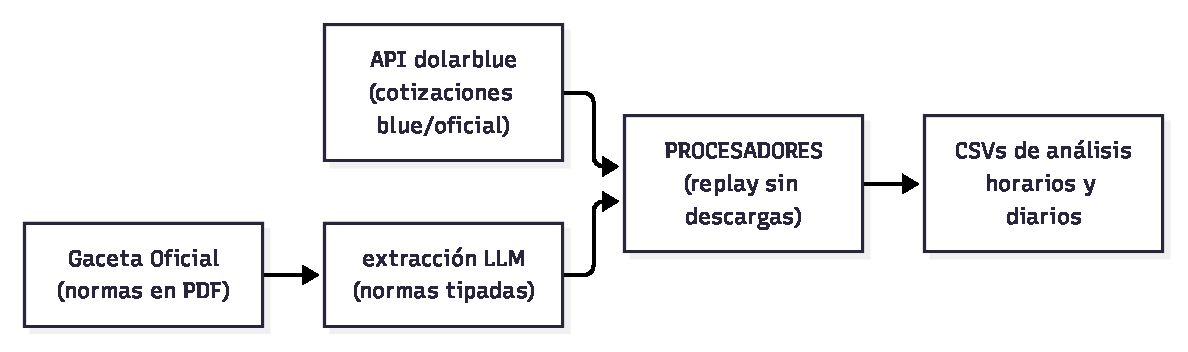
\includegraphics[width=\textwidth]{diagram_flujo_datos.pdf}
\caption{Obtención de datos: las dos fuentes convergen en los procesadores,
que producen los CSVs de análisis.}
\label{fig:flujo_datos}
\end{figure}

\subsection{Trazabilidad del pipeline}

La figura~\ref{fig:pipeline_anim} es el fotograma final de una animación de
60 segundos que recorre la extracción, los indexers y la exploración de las
dos fuentes. El video está en \texttt{report/anim/pipeline.mp4} (y la versión
GIF en \texttt{report/anim/pipeline.gif}); se regenera con
\texttt{make anim}.
Las escenas 5 y 6 detallan los dos indexers: el horario deriva precios medios,
spread, brecha, retorno y volatilidad; el diario construye un calendario
completo y rellena con cero los días sin publicación. La escena 7 muestra la
interpolación de huecos de hasta 3~h y las reglas para el resto. El notebook
(sección~2.2) y el dashboard (sección~3.6) reproducen las ocho escenas como
clips animados, con el frame final como respaldo.

La animación muestra el comportamiento efectivo del código. La corrida se
protege con un manifiesto de 24 h; cada PDF se reutiliza si ya está en disco
(más de 1~KB, validado por tamaño) y la extracción LLM se cachea por
\texttt{sha256(pdf):provider:model}; la firma \texttt{\%PDF} se exige en las
descargas nuevas. Un fallo de descarga o de esquema se
reintenta hasta tres veces con retroceso; si persiste, no se cachea y queda
para la corrida siguiente. La etiqueta \texttt{relevancia\_fx} es una salida:
una norma \texttt{nula} se conserva con peso cero y no se reintenta. En la
serie horaria, un único hueco de 3~h se interpola ($\le 3$~h); los huecos
mayores y el calentamiento de \texttt{vol\_24h} quedan como \texttt{NaN}, y
los días sin norma en la Gaceta son ceros estructurales, no datos faltantes.

\begin{figure}[!ht]
\centering
\includegraphics[width=\textwidth]{fig_pipeline_poster.pdf}
\caption{Fotograma final de la animación del pipeline: descarga única, cache
de extracción, reintento acotado y faltantes explícitos. El video completo
está en \texttt{report/anim/pipeline.mp4}.}
\label{fig:pipeline_anim}
\end{figure}

\subsection{Fuentes de datos}

Las fuentes del proyecto son la API pública de cotizaciones del dólar blue
\cite{dolarblue2026api} y las normas publicadas en la Gaceta Oficial de
Bolivia \cite{gaceta2026}.

La API expone tres categorías: cotizaciones al instante (nivel oficial y
libros P2P), series históricas por hora de 6 meses e historial completo
exportable.

\subsection{Diccionario de datos}

El modelado se alimenta de tres archivos. La tabla~\ref{tab:diccionario}
resume las variables que se usan y su unidad.

\begin{table}[!ht]
\centering\footnotesize
\begin{tabular}{@{}p{0.19\textwidth}p{0.34\textwidth}p{0.39\textwidth}@{}}
\toprule
Archivo & Variable & Contenido (unidad) \\
\midrule
\texttt{market\_hourly.csv} & & \emph{frecuencia horaria, 4\,318 filas} \\
 & \texttt{fecha} & marca horaria en UTC \\
 & \texttt{blue\_mid}, \texttt{oficial\_mid} & punto medio (compra$+$venta)/2
   del blue y del oficial (Bs/USD) \\
 & \texttt{brecha\_pct} & brecha blue--oficial sobre el oficial (\%) \\
 & \texttt{spread\_blue} & venta menos compra del blue (Bs/USD) \\
 & \texttt{ret\_blue\_1h} & retorno horario del blue (\%) \\
 & \texttt{vol\_24h} & desvío estándar móvil de 24~h de los retornos \\
\midrule
\texttt{panel\_diario.csv} & & \emph{179 días, cruce mercado $\times$ Gaceta} \\
 & \texttt{n\_docs\_fx}, \texttt{n\_docs\_fx\_alta} & normas del día con
   relevancia cambiaria media/alta y alta (conteo) \\
 & \texttt{n\_docs\_deuda}, \texttt{n\_docs\_comercio}, \texttt{n\_docs\_mineria}
   & normas del día por canal temático (conteo) \\
 & \texttt{vol\_media\_24h} & volumen P2P medio del día (USD) \\
 & \texttt{d\_oficial\_pct} & variación diaria del oficial (\%) \\
\midrule
\texttt{gaceta\_llm.csv} & & \emph{169 normas, una fila por documento} \\
 & \texttt{relevancia\_fx} & nula, baja, media o alta (categoría) \\
 & \texttt{tags} & canales temáticos asignados por el LLM \\
 & \texttt{monto\_usd} & monto explícito en dólares, si la norma lo declara \\
 & \texttt{confidence} & confianza de la extracción, entre 0 y 1 \\
\midrule
\emph{Derivadas} & \texttt{brecha\_lag1h}, \texttt{lag3h}, \texttt{lag24h},
   \texttt{oficial\_lag1h}, \texttt{vol\_lag1h}, \texttt{ret\_blue\_lag1h},
   \texttt{n\_docs\_*\_lag1} & rezagos usados como predictores (la Gaceta entra
   rezagada un día) \\
 & \texttt{hora\_*}, \texttt{dow\_*} & dummies de hora (23) y de día de la
   semana (6) \\
\bottomrule
\end{tabular}
\caption{Variables usadas por el modelado, por archivo.}
\label{tab:diccionario}
\end{table}

\subsection{Exploración (EDA)}
\label{sec:analisis}

La exploración usa la serie horaria de \textbf{4\,321 horas}
(2026-04-27 02:00 $\rightarrow$ 2026-10-24 02:00) y, para la brecha diaria,
la serie de \textbf{366 días} (2025-10-24 $\rightarrow$ 2026-10-24). El panel
que incorpora los canales de la Gaceta cubre \textbf{179 días}
(2026-04-29 $\rightarrow$ 2026-10-24).

\subsubsection{Serie blue vs oficial}

La \hyperref[fig:serie]{figura~\ref*{fig:serie}} muestra la serie por hora de
los últimos $\sim$6 meses (\texttt{chart\_6m.csv}): compra/venta del dólar
blue frente al oficial BCB. Se aprecia el tipo de cambio administrado (oficial
prácticamente plano) contra la flotación libre del paralelo.

\begin{figure}[!ht]
\centering
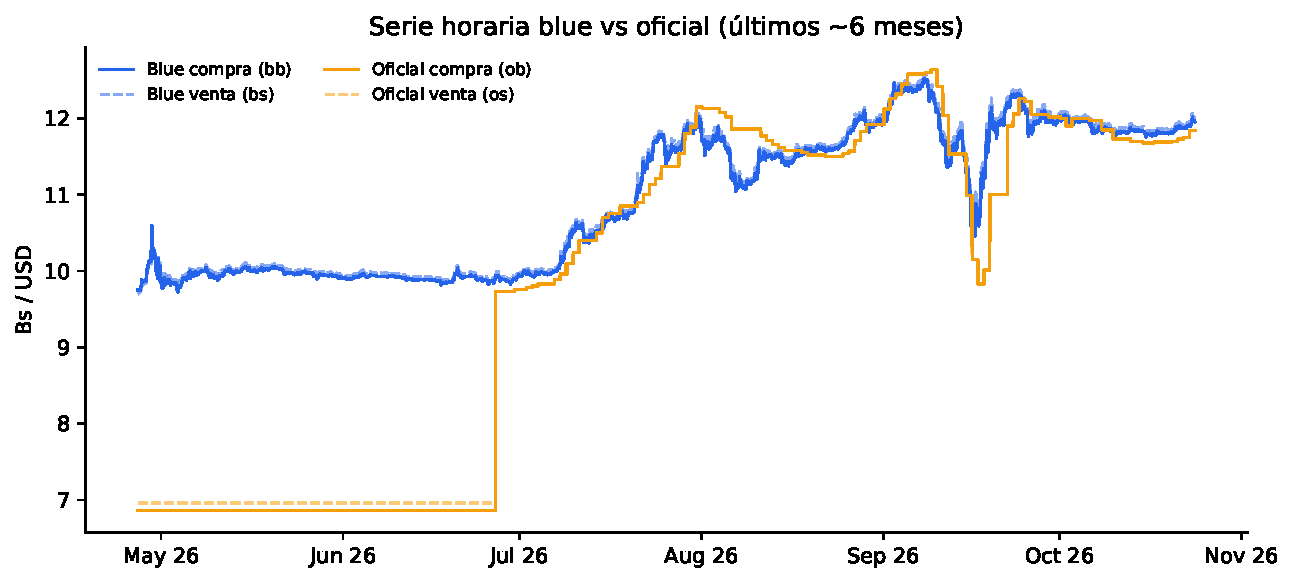
\includegraphics[width=\textwidth]{fig_serie_blue_oficial.pdf}
\caption{Serie por hora blue vs oficial (compra/venta), últimos $\sim$6 meses.}
\label{fig:serie}
\end{figure}

\subsubsection{La brecha cambiaria}

La \hyperref[fig:brecha]{figura~\ref*{fig:brecha}} resume la brecha diaria
(precio medio blue $-$ precio medio oficial) construida desde
\texttt{history\_full.csv} con resampleo diario. Es la base de la variable
objetivo de predicción (Objetivos 1--2, \hyperref[sec:preparacion]{sección~\ref*{sec:preparacion}}).

\begin{figure}[!ht]
\centering
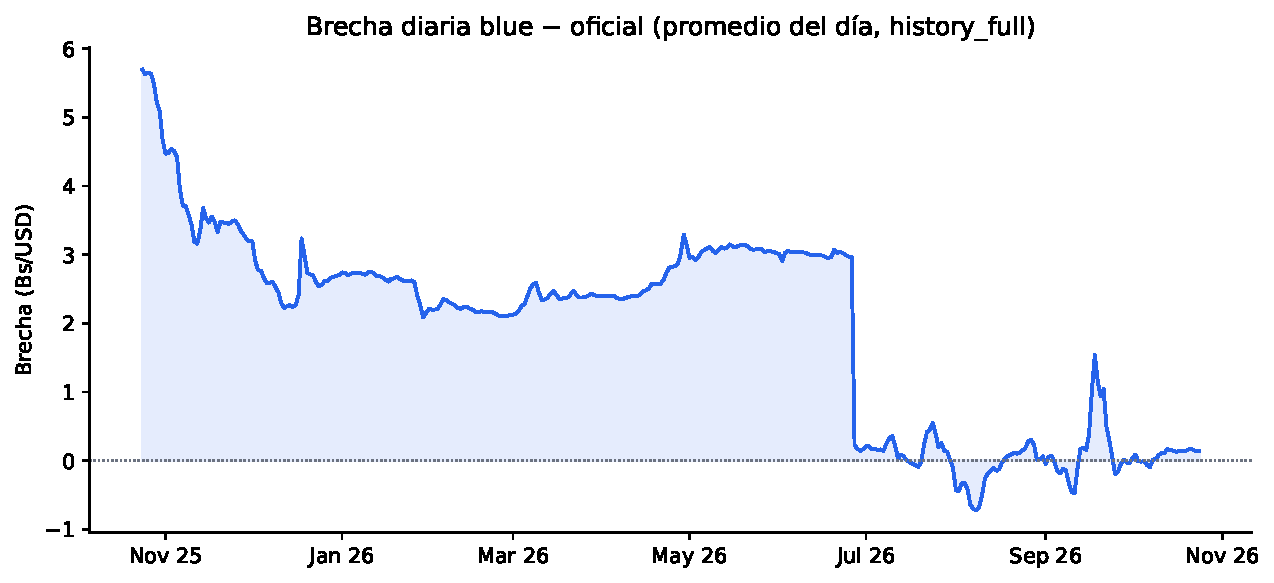
\includegraphics[width=\textwidth]{fig_brecha.pdf}
\caption{Brecha diaria blue $-$ oficial (promedio del día).}
\label{fig:brecha}
\end{figure}

\begin{table}[!ht]
\centering
% Generado por make_figures.py — no editar a mano
\begin{tabular}{@{}lll@{}}
\toprule
Métrica & Valor & Unidad \\
\midrule
Puntos horarios & 4.318 &  \\
Blue medio & 10,98 & Bs/USD \\
Oficial medio & 9,90 & Bs/USD \\
Spread blue medio (bs$-$bb) & 0,05 & Bs/USD \\
Volatilidad diaria blue ($\sigma$ de retornos) & 0,20 & \% \\
Días de brecha (history\_full) & 366 &  \\
Brecha media & 1,94 & Bs/USD \\
Brecha máxima & 5,70 & Bs/USD \\
\bottomrule
\end{tabular}

\caption{Métricas de la serie vigente (blue vs oficial, brecha y
volatilidad).}
\label{tab:resumen}
\end{table}


\subsection{Calidad de datos}

Sobre \textbf{34\,182 snapshots} se descartó un único registro con precio nulo;
la serie horaria requiere interpolar un único hueco de 3~h. La Gaceta tiene
\textbf{169 normas} extraídas con LLM (2026-06-18 $\rightarrow$ 10-20) más
\textbf{509} etiquetadas por palabras clave como respaldo (2025-10-12
$\rightarrow$ 10-07); aun así, solo \textbf{23 de los 179 días} del panel
tienen alguna norma con relevancia cambiaria. En el cruce temporal, 117 de los
249 pares fecha--tag del estudio de eventos tienen datos de mercado.
          % incluye 2.4 Exploración (04_analisis)
\section{Preparación de datos}
\label{sec:preparacion}

Esta fase transforma las fuentes crudas descritas en la
\hyperref[sec:datos]{sección~\ref*{sec:datos}} en una tabla lista para
modelar, con el objetivo de \textbf{predecir} el nivel del paralelo y la
brecha oficial--paralelo a horizontes cortos. El énfasis del proyecto está en
la previsión, no en el monitoreo en tiempo real: cada decisión de
preparación se toma pensando en evitar fuga de información y en reproducir el
orden temporal real de los datos.

\subsection{Del JSON crudo a los predictores del modelo}

El camino desde la API hasta los predictores tiene cuatro etapas:

\begin{enumerate}
  \item \textbf{Recolección.} Un colector consulta el endpoint
        \texttt{GET /v1/chart/6m} de la API y guarda cada respuesta como
        snapshot JSON en \texttt{data/raw/}: una lista de puntos muestreados
        cada hora.
  \item \textbf{Normalización.} Se elimina el envoltorio de la API y cada
        punto se valida contra un esquema tipado; el resultado se escribe en
        \texttt{data/normalized/chart\_6m.csv}. Toda la API se reduce a
        5 columnas: \texttt{t} (epoch, una fila por hora), \texttt{bb}/\texttt{bs}
        (blue compra/venta, Bs/USD) y \texttt{ob}/\texttt{os} (oficial
        compra/venta).
  \item \textbf{Ingeniería de características.} Una etapa de indexación deriva
        los puntos medios, el spread, la brecha porcentual, el retorno por hora
        y la volatilidad rodante de 24~h; las columnas \texttt{fwd\_*} son
        retornos futuros (etiquetas de previsión, no predictores). Resultado:
        \texttt{data/processed/market\_hourly.csv} (4\,315 filas
        $\times$ 17 columnas).
  \item \textbf{Predictores del modelo.} Los modelos lineales consumen
        rezagos de esos campos más los canales de la Gaceta:
        \begin{itemize}
          \item \textbf{Variante por hora (37 predictores):} rezagos de brecha
                (1, 3 y 24~h), oficial, volatilidad y retorno (todos con
                \texttt{shift(1)}, sin fuga); canales de la Gaceta contados
                por día (\texttt{n\_docs\_fx}, \texttt{n\_docs\_fx\_alta},
                sobre 509 normas etiquetadas por palabras clave) y
                transmitidos a cada hora del día siguiente;
                dummies de hora (23) y de día de semana (6).
        \end{itemize}
\end{enumerate}

\subsection{Remuestreo a frecuencia fija}

Las fuentes no son uniformes: \texttt{history\_full.csv} registra snapshots
por eventos y los exchanges cambian de periodicidad. Todo se alinea a una
\textbf{frecuencia horaria} (4\,321 filas): se conserva el último precio
observado y se interpolan huecos de hasta 3 períodos. La frecuencia diaria se usa
solo para los canales de la Gaceta, que tienen resolución de publicación.


\subsection{Variable objetivo y conjunto de eventos}

El problema se formula como \textbf{previsión supervisada} a dos horizontes:
el nivel del paralelo (o la brecha) \textbf{a una hora y a un día}, con
intervalos que cuantifiquen la incertidumbre. Para cada horizonte $h$ los
predictores usan solo información disponible en $t-h$, y la línea base naïve
repite el último valor observado en ese origen. Para el Objetivo~2 se cruza la serie horaria con las fechas de
edición de la Gaceta: por cada publicación se toma el precio ancla (12:00~UTC)
y se miden retornos a 5~h, 1, 3 y 5 días contra la variación media de todos los
días de la serie (línea base incondicional).

\subsection{Partición temporal y línea base}

La partición respeta el orden temporal, nunca una división aleatoria: el
ventana de prueba es el \textbf{último corte temporal} (las últimas 168~h), el mismo
para todos los modelos. Se define una
\textbf{línea base naïve} (último valor observado, equivalente al paseo
aleatorio) que todo modelo debe superar fuera de muestra: en tipos de cambio
es un referente notoriamente difícil de batir.

\section{Modelado}
\label{sec:modelado}

Se ajustan dos objetivos sobre las tablas de la fase~3: predecir el nivel del
paralelo y la brecha (\textbf{Objetivo 1}) y medir la relación entre la Gaceta y
la brecha (\textbf{Objetivo 2}). La entrada es la serie horaria (\textbf{4\,321
h}) y el panel diario de \textbf{179 días} con los canales de la Gaceta.

\textbf{Quiebre estructural.} La muestra tiene un solo quiebre: la devaluación
del oficial el \textbf{2026-06-27} (6{,}91 $\rightarrow$ 9{,}73~Bs/USD, $+41\%$).
La ventana de prueba cae íntegra después, así que las métricas miden el período
vigente. El ARIMA se entrena con los 90 días posteriores al quiebre; la regresión
y el HAC usan las 4\,128~h completas.

\subsection{Diseño de validación}

\begin{itemize}
  \item \textbf{Partición temporal fija:} las últimas 168 h, mismo corte para
        todos los modelos.
  \item \textbf{Dos horizontes:} 1 hora y 1 día, con origen móvil y el naïve
        del mismo horizonte como línea base
        \cite{makridakis2020m4}.
  \item \textbf{Métricas:} RMSE y MAE en unidades del target, y su cociente
        frente al naïve.
\end{itemize}

\subsection{Regresión lineal múltiple (predicción)}

Nivel de la brecha y del paralelo sobre \textbf{37 predictores} sin fuga de
información: rezagos (1, 3 y 24~h), oficial y volumen P2P rezagados, los dos
canales cambiarios de la Gaceta a un día y dummies de hora y de día de semana.

\begin{table}[!ht]
\centering\small
\begin{tabular}{@{}llcccc@{}}
\toprule
Target & Horizonte & RMSE & MAE & naïve & RMSE $\div$ naïve \\
\midrule
Brecha (pp)   & 1~h  & 0{,}1175 & 0{,}073 & 0{,}0910 & 1{,}29 \\
              & 24~h & 0{,}886  & 0{,}550 & 0{,}2350 & 3{,}77 \\
Paralelo (Bs) & 1~h  & 0{,}0819 & 0{,}081 & 0{,}0077 & 10{,}6 \\
              & 24~h & 0{,}126  & 0{,}119 & 0{,}0390 & 3{,}22 \\
\bottomrule
\end{tabular}
\caption{Regresión lineal múltiple en la ventana de prueba de 168~h, a dos
horizontes. En cada caso el naïve es el último valor observado en el origen del
pronóstico: $y(t-1)$ para 1~h e $y(t-24)$ para 24~h.}
\label{tab:rl_multiple}
\end{table}

\begin{figure}[!ht]
\centering
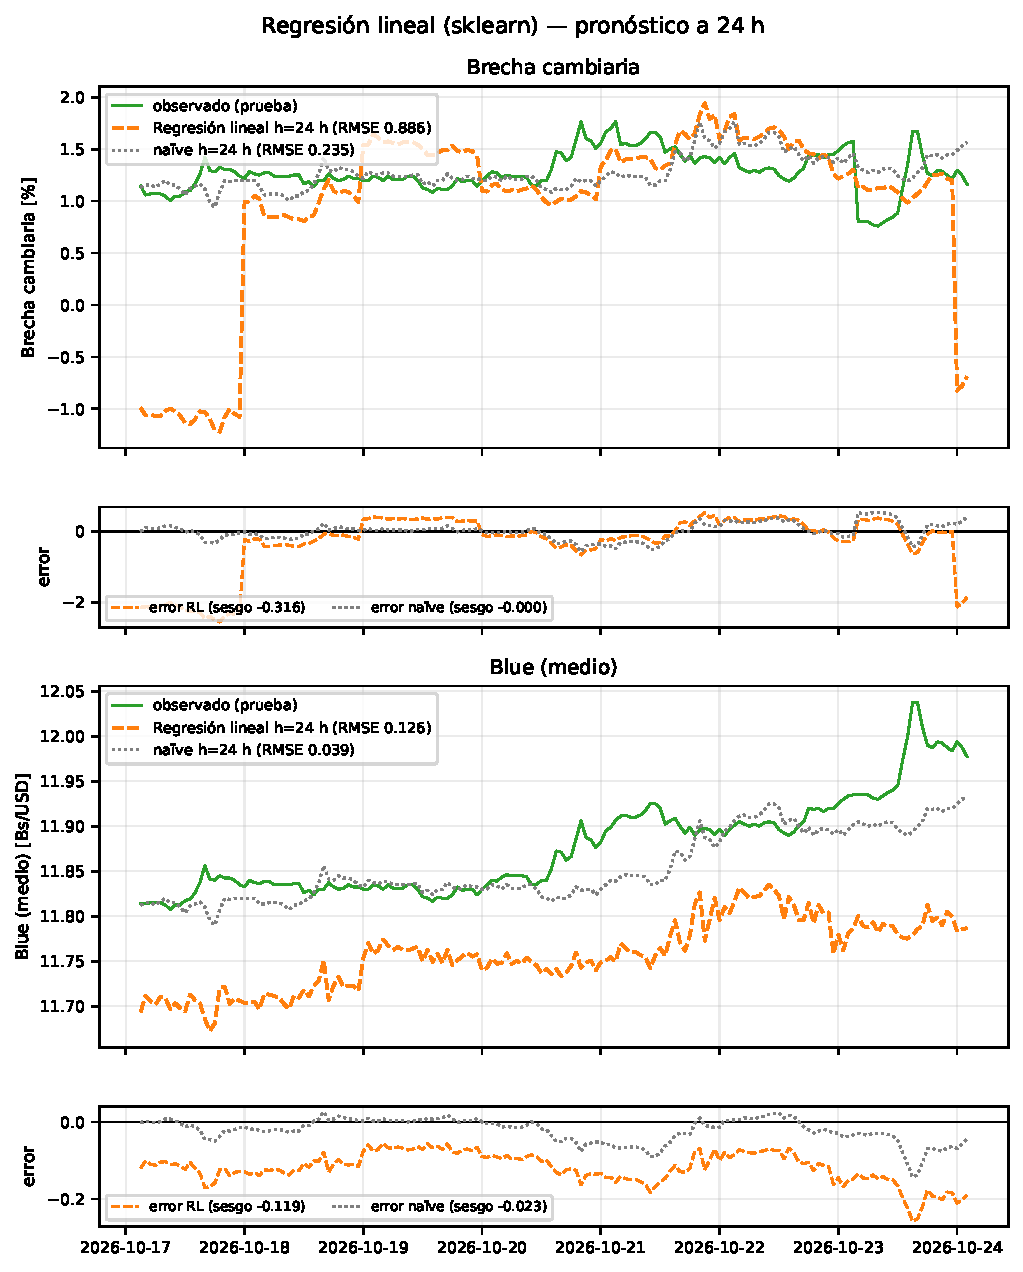
\includegraphics[width=\textwidth]{fig_rl_test.pdf}
\caption{Regresión lineal múltiple a una hora (columna izquierda) y a un día
(columna derecha) frente al observado y al naïve, en la ventana de prueba
(168~h). Cada columna muestra, para la brecha y el nivel del blue, el nivel
(arriba) y el \textbf{error} (predicción $-$ observado, abajo), con su sesgo
medio. A 24~h el error de nivel es casi constante ($-0{,}119$~Bs: predice
sistemáticamente por debajo); en la brecha el modelo se desborda en los extremos
(llega a $-2{,}5$\,pp cuando el rango observado es $0{,}8$--$1{,}8$), que es el
origen de su RMSE de $0{,}886$. A una hora el sesgo también es negativo
($-0{,}081$~Bs) y el RMSE del nivel multiplica por $10{,}6$ al del naïve.}
\label{fig:rl_test}
\end{figure}

\textbf{Lectura.} La regresión \textbf{pierde contra el naïve en los cuatro
casos}. A una hora el nivel es casi un paseo aleatorio: repetir la hora anterior
deja un error de $0{,}0077$~Bs ($0{,}07$\,\% del precio) y el modelo, con su
sesgo de nivel, llega a $0{,}0819$. A un día ambos se degradan, pero la brecha
empeora mucho más ($0{,}886$ contra $0{,}235$).

\FloatBarrier
\subsection{OLS con errores HAC (inferencia)}

El mismo diseño se reestima con \textbf{errores HAC de Newey--West} (24
rezagos, un ciclo diario), robustos a heterocedasticidad y autocorrelación: los
$\beta$ no cambian, cambia el error estándar.


\begin{table}[!ht]
\centering\small
\begin{tabular}{@{}lcccc@{}}
\toprule
Coeficiente & $\beta$ & ee HAC & $p$-valor & IC 95\% \\
\midrule
\texttt{brecha\_lag1h}  & 0{,}9899 & 0{,}0064 & $<0{,}001$ & $[0{,}9773;\,1{,}0024]$ \\
\texttt{oficial\_lag1h} & $-0{,}0263$ & 0{,}0098 & 0{,}0075 & $[-0{,}0456;\,-0{,}0070]$ \\
\bottomrule
\end{tabular}
\caption{Coeficientes significativos al 5\% (OLS + HAC sobre la brecha
horaria; $R^2$ dentro de muestra $= 0{,}9987$, $n = 4\,128$).}
\label{tab:ols_hac}
\end{table}

\begin{figure}[!ht]
\centering
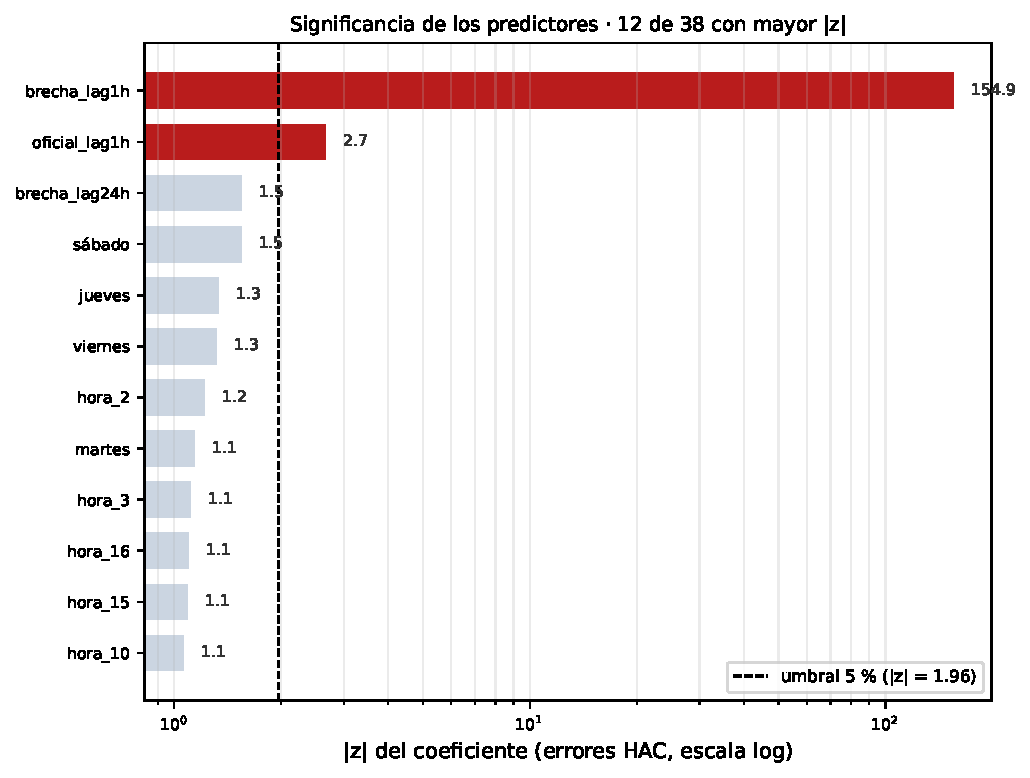
\includegraphics[width=\textwidth]{fig_hac_z.pdf}
\caption{Significancia de los coeficientes HAC: solo \texttt{brecha\_lag1h} y
\texttt{oficial\_lag1h} superan el umbral del 5\,\%; el resto tiene $|z|$
cercano a 1 (escala logarítmica).}
\label{fig:hac_z}
\end{figure}

\textbf{Lectura.} Solo dos coeficientes son significativos:
\texttt{brecha\_lag1h} ($\approx 0{,}99$, persistencia casi perfecta) y
\texttt{oficial\_lag1h} ($-0{,}026$, efecto denominador). \textbf{Ningún canal
de la Gaceta ni el volumen} resultan significativos, coherente con la
sección~4.6.

\FloatBarrier
\subsection{ARIMA}

\paragraph{Selección del orden.} El orden $(p,d,q)$ se eligió por el
\emph{criterio de información de Akaike} (AIC), calculado \textbf{solo con el
entrenamiento}, sobre una grilla con $p,q \le 2$ y $d \in \{0,1\}$
\cite{box2015timeseries}. El AIC elige ARIMA($2{,}1{,}1$) para el nivel y
ARIMA($2{,}1{,}2$) para la brecha.

La selección se repite \textbf{por horizonte}, con la ventana de entrenamiento
que corresponde a cada uno: el origen inicial de un pronóstico a $h$ pasos está
$h$ horas antes del primer objetivo, de modo que el modelo a un día no ve las
últimas 23~h de la muestra. El orden no cambia, pero el AIC sí ($-9\,305{,}0$ a
1~h y $-9\,301{,}2$ a 24~h en el nivel; $2\,926{,}5$ y $2\,931{,}4$ en la
brecha).

\begin{table}[!ht]
\centering\small
\begin{tabular}{@{}lccc@{}}
\toprule
Orden & tendencia & AIC \texttt{blue\_mid} & AIC \texttt{brecha\_pct} \\
\midrule
$(0,0,1)$ & constante & -916{,}9 & 8\,909{,}8 \\
$(0,0,2)$ & constante & -3\,121{,}2 & 7\,241{,}5 \\
$(1,0,0)$ & constante & -9\,210{,}3 & 2\,944{,}7 \\
$(1,0,1)$ & constante & -9\,299{,}4 & 2\,946{,}4 \\
$(1,0,2)$ & constante & -9\,299{,}0 & 2\,948{,}0 \\
$(2,0,0)$ & constante & -9\,291{,}8 & 2\,946{,}4 \\
$(2,0,1)$ & constante & -9\,302{,}6 & 2\,931{,}6 \\
$(2,0,2)$ & constante & -9\,297{,}5 & 2\,929{,}7 \\
$(0,1,1)$ & sin deriva & -9\,303{,}7 & 2\,948{,}2 \\
$(0,1,2)$ & sin deriva & -9\,304{,}2 & 2\,949{,}5 \\
$(1,1,0)$ & sin deriva & -9\,296{,}4 & 2\,948{,}2 \\
$(1,1,1)$ & sin deriva & -9\,304{,}6 & 2\,933{,}8 \\
$(1,1,2)$ & sin deriva & -9\,304{,}5 & 2\,931{,}0 \\
$(2,1,0)$ & sin deriva & -9\,299{,}6 & 2\,949{,}8 \\
$(2,1,1)$ & sin deriva & \textbf{-9\,305{,}0} & 2\,930{,}1 \\
$(2,1,2)$ & sin deriva & -9\,303{,}7 & \textbf{2\,926{,}5} \\
\bottomrule
\end{tabular}
\caption{Grilla completa: 16 candidatos con $p,q \le 2$ y $d \in \{0,1\}$
(constante si $d=0$, sin deriva si $d=1$). En negrita el mínimo de cada serie.
La grilla se calcula solo con entrenamiento ($n = 2\,160$) y se repite para cada
horizonte.}
\label{tab:arima_grid}
\end{table}

\begin{table}[!ht]
\centering\small
\begin{tabular}{@{}llcccc@{}}
\toprule
Target & Horizonte & RMSE & MAE & naïve & RMSE $\div$ naïve \\
\midrule
\texttt{blue\_mid} (Bs)   & 1~h  & \textbf{0{,}0074} & 0{,}0050 & 0{,}0077 & 0{,}96 \\
                          & 24~h & 0{,}0390 & 0{,}0277 & 0{,}0390 & 1{,}00 \\
\texttt{brecha\_pct} (pp) & 1~h  & 0{,}0907 & 0{,}0492 & 0{,}0910 & 1{,}00 \\
                          & 24~h & 0{,}2338 & 0{,}1786 & 0{,}2350 & 0{,}99 \\
\bottomrule
\end{tabular}
\caption{ARIMA en la ventana de prueba de 168~h, a dos horizontes, con
evaluación de origen móvil: para cada hora objetivo se pronostica desde
$t-h$ y el modelo se actualiza con los valores reales. El naïve es el último
valor observado en el origen. El orden se reselecciona por horizonte con AIC
sobre la ventana de entrenamiento correspondiente (2\,160~h): resulta
ARIMA(2,1,1) para el nivel y ARIMA(2,1,2) para la brecha en ambos casos.}
\label{tab:arima}
\end{table}

\begin{figure}[!ht]
\centering
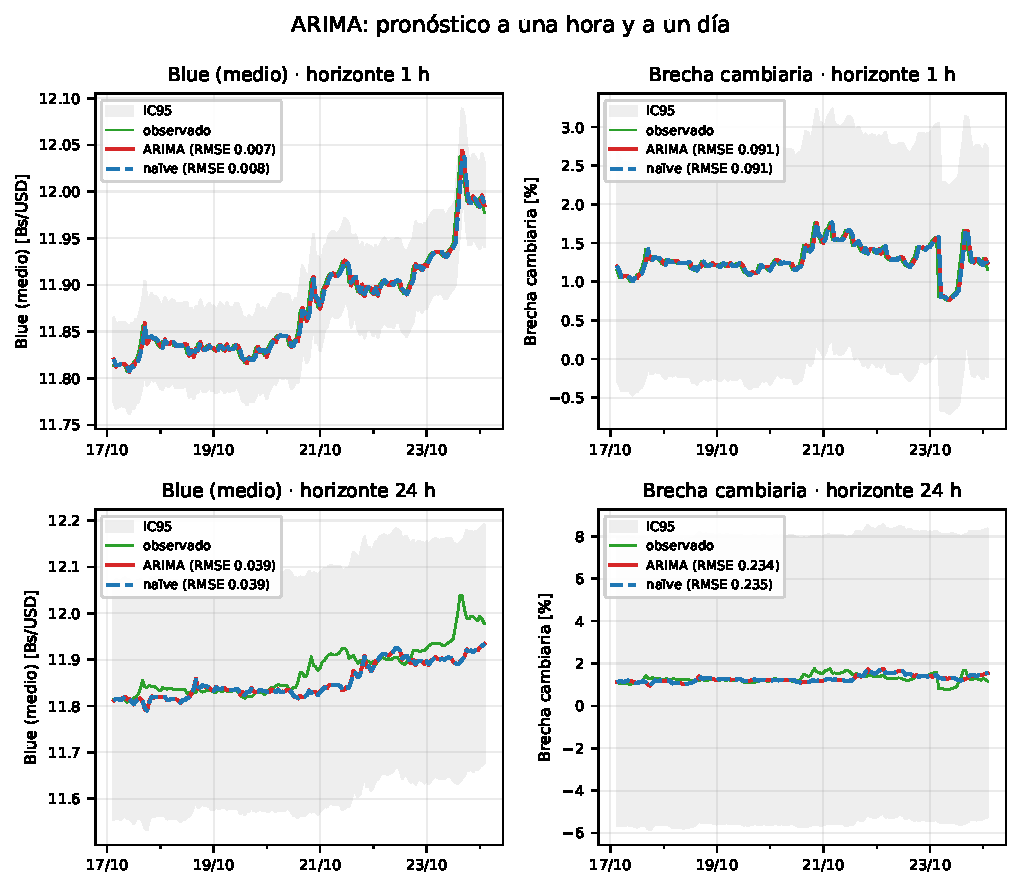
\includegraphics[width=\textwidth]{fig_arima_test.pdf}
\caption{ARIMA en la ventana de prueba (168~h) en los dos horizontes: fila
superior a una hora, fila inferior a un día. La columna izquierda es el nivel
del blue y la derecha la brecha. A una hora el pronóstico sigue de cerca al
observado y la banda es estrecha; a un día la línea del modelo se separa y la
banda se ensancha hasta cubrir casi todo el rango. En ambos casos la línea del
ARIMA anda muy cerca de la del naïve: sin deriva, el pronóstico puntual de un
paseo aleatorio es el último valor observado, y lo que aporta el modelo es la
banda de incertidumbre.}
\label{fig:arima_test}
\end{figure}

\textbf{Lectura.} El ARIMA \textbf{iguala o mejora levemente al naïve en los
cuatro casos}: a una hora reduce el RMSE del nivel un $4{,}5$\,\% y a un día las
diferencias son de una décima de punto. El valor del modelo no está en acertar
más ---el tipo de cambio horario se comporta como un paseo aleatorio
--- sino en la banda de incertidumbre.

\FloatBarrier
\subsection{Comparativa del Objetivo 1}

\begin{table}[H]
\centering\small
\begin{tabular}{@{}llccccc@{}}
\toprule
 & & & \multicolumn{2}{c}{RMSE} & \multicolumn{2}{c}{MAE} \\
\cmidrule(lr){4-5}\cmidrule(l){6-7}
Target & Horizonte & Modelo & valor & $\div$ naïve & valor & $\div$ naïve \\
\midrule
Brecha (pp)   & 1~h  & ARIMA(2{,}1{,}2) & \textbf{0{,}0907} & 1{,}00 & \textbf{0{,}0492} & 1{,}00 \\
              &      & RL múltiple      & 0{,}1175 & 1{,}29 & 0{,}0730 & 1{,}48 \\
              & 24~h & ARIMA(2{,}1{,}2) & \textbf{0{,}2338} & 0{,}99 & \textbf{0{,}1786} & 0{,}99 \\
              &      & RL múltiple      & 0{,}886  & 3{,}77 & 0{,}5504 & 3{,}05 \\
\midrule
Paralelo (Bs) & 1~h  & ARIMA(2{,}1{,}1) & \textbf{0{,}0074} & 0{,}96 & \textbf{0{,}0050} & 1{,}00 \\
              &      & RL múltiple      & 0{,}0819 & 10{,}6 & 0{,}0809 & 16{,}2 \\
              & 24~h & ARIMA(2{,}1{,}1) & \textbf{0{,}0390} & 1{,}00 & \textbf{0{,}0277} & 1{,}00 \\
              &      & RL múltiple      & 0{,}126  & 3{,}22 & 0{,}1191 & 4{,}30 \\
\bottomrule
\end{tabular}
\caption{Resumen del Objetivo 1 (ventana de prueba de 168~h), a los dos
horizontes, en RMSE y MAE. El cociente $\div$ naïve $=1$ es empate; valores
mayores indican peor desempeño. Cada modelo se compara con el naïve de su mismo
horizonte. El MAE es la magnitud que entra en el costo de operación
(sección~\ref{sec:negocio_eval}).}
\label{tab:comparativa}
\end{table}

\textbf{Lectura.} El \textbf{ARIMA domina a la regresión en los cuatro
pares} y es el único que no pierde contra su línea base: iguala al naïve a un
día ($0{,}99$--$1{,}00$) y lo mejora levemente a una hora en el nivel
($0{,}96$). La regresión múltiple, en cambio, pierde en todos los casos, con el
caso extremo del nivel a 1~h ($10{,}6\times$ en RMSE y $16{,}2\times$ en MAE).

Las dos métricas coinciden en el ordenamiento, pero el MAE matiza dos
resultados. En el nivel a una hora el ARIMA iguala al naïve en MAE ($1{,}00$)
aunque lo supere en RMSE ($0{,}96$): la ganancia está en las horas atípicas, no
en el error típico, y por eso \textbf{no se traduce en ahorro} en la
sección~\ref{sec:negocio_eval}. Y en la brecha la regresión pierde más en MAE
($1{,}48$) que en RMSE ($1{,}29$), señal de que la diferencia entre ambos se
estrecha en las horas de salto, donde el naïve acumula sus errores más grandes. El patrón es consistente con la
naturaleza de la serie: el valor de la hora anterior contiene casi toda la
información, y un modelo con 37 predictores estimados sobre seis meses no
alcanza a explotarla mejor que una regla trivial. El margen de aporte está en
la incertidumbre (sección~\ref{sec:negocio_eval}), no en el error puntual.

\FloatBarrier
\subsection{Objetivo 2 --- Publicaciones de la Gaceta y brecha}

\subsubsection{Estudio de eventos por tag}

Para cada fecha de edición de la Gaceta se toma el \texttt{blue\_mid} de las
12:00~UTC como ancla y se mide la variación porcentual a cuatro horizontes: 5
horas, 1, 3 y 5 días. Cada par (fecha, tag) es un evento; el benchmark es la
variación media de \emph{todos} los días de la serie horaria al mismo
horizonte (la deriva propia de la muestra), y el \textbf{exceso}
($\text{evento} - \text{benchmark}$) es lo interpretable como efecto de la
publicación. La serie horaria cubre 181 días (2026-04-27 $\rightarrow$
10-24), de modo que 117 de los 249 pares fecha--tag tienen datos de mercado.

\begin{table}[!ht]
\centering\small
\begin{tabular}{@{}lrrrrr@{}}
\toprule
Tag & $n$ & 5 h (pp) & 1 d (pp) & 3 d (pp) & 5 d (pp) \\
\midrule
\texttt{divisas\_control\_cambios} & 5  & $-0{,}28$ & $-0{,}31$ & $+0{,}05$ & $+0{,}95$ \\
\texttt{deuda\_externa}            & 6  & $-0{,}20$ & $+0{,}05$ & $+0{,}19$ & $+0{,}87$ \\
\texttt{comercio\_exterior}        & 12 & $-0{,}05$ & $+0{,}34$ & $+0{,}51$ & $+1{,}33$ \\
\texttt{general\_administrativo}   & 42 & $+0{,}01$ & $+0{,}26$ & $+1{,}03$ & $+1{,}21$ \\
\texttt{mineria\_energia}          & 18 & $+0{,}17$ & $+0{,}34$ & $+0{,}03$ & $+0{,}21$ \\
\texttt{impuestos}                 & 22 & $+0{,}18$ & $+0{,}37$ & $+0{,}57$ & $+1{,}05$ \\
\texttt{credito\_financiero}       & 7  & $+0{,}19$ & $+0{,}66$ & $+1{,}06$ & $+1{,}32$ \\
\texttt{fiscal\_presupuesto}       & 4  & $+0{,}50$ & $+1{,}06$ & $+3{,}83$ & $+3{,}38$ \\
\texttt{contrataciones\_estado}    & 1  & $+0{,}12$ & $+0{,}29$ & $+0{,}04$ & $+0{,}14$ \\
\bottomrule
\end{tabular}
\caption{Exceso de variación del blue sobre la línea base incondicional, por
tag y horizonte (ordenado por efecto a 5~h). También
\texttt{general\_administrativo} cruza el umbral a 3--5 días, pero es el
conjunto no cambiario: no respalda la hipótesis.}
\label{tab:eventos}
\end{table}

\textbf{Lectura.} Los tags cambiarios (\texttt{divisas\_control\_cambios},
\texttt{deuda\_externa}) son los únicos con exceso negativo a 5~h --- la
dirección que predice la hipótesis ---: \texttt{divisas} lo mantiene también a
1~día ($-0{,}31$), mientras \texttt{deuda} cambia de signo. Ninguno es
significativo con $n \geq 5$ en los horizontes cambiarios. El caso
\texttt{fiscal\_presupuesto} ($+3{,}8$~pp a 3~d) es ruido: $n=4$ y un IC95 de
$\pm7{,}2$~pp.

\subsubsection{Correlación diaria (Spearman)}

Por día se cuenta cuántas normas de cada tag se publicaron y se cruza con el
retorno diario del blue, en el mismo día ($t$) y con un día de rezago
($t{+}1$). Se usa Spearman y no Pearson porque el conteo diario es discreto y
muy sesgado hacia cero, y el retorno tiene valores atípicos; la correlación de
rangos es robusta a ambos problemas.

\textbf{Lectura.} Todas las correlaciones son débiles ($|\rho| \leq 0{,}16$):
no hay relación monótona apreciable entre la intensidad de publicación de
ningún tag y el retorno diario del blue.

\FloatBarrier
\subsection{Limitaciones}

\begin{itemize}
  \item \textbf{Una sola semana de prueba:} el RMSE depende de pocas horas
        atípicas y las diferencias entre modelos no son concluyentes con esta
        muestra.
  \item \textbf{Gaceta dispersa:} solo \textbf{23 de 179 días} tienen una norma
        con relevancia cambiaria, y por eso ningún canal resulta significativo.
\end{itemize}

\section{Evaluación de negocio}
\label{sec:negocio_eval}

Esta sección traduce las métricas de la fase~4 a decisiones, siguiendo la fase~5
de CRISP-DM.

\subsection{El error de nivel no genera ahorro}

El error que importa en una operación de compra/venta es el MAE en Bs por USD
multiplicado por el monto operado. A una hora el ARIMA y el naïve empatan
(\textbf{0{,}0050}~Bs/USD) y a un día también (\textbf{0{,}0277}): \textbf{el
ahorro por precisión es cero a cualquier volumen}. La única diferencia medible
es el RMSE a una hora, $4{,}5$\,\% mejor, y no se traduce en ahorro porque el
MAE es idéntico.

\subsection{La señal direccional solo sirve a una hora}

Si el modelo se usa para decidir \emph{cuándo} comprar, lo que pesa es la
asimetría entre comprar y que baje (falso positivo) y no comprar y que suba
(falso negativo), no el error medio. Las matrices usan las predicciones de origen
móvil de la sección~4.4:

\begin{table}[!ht]
\centering\small
\begin{tabular}{@{}llcc@{}}
\toprule
Horizonte & & predice sube & predice baja \\
\midrule
1~h  & real sube & 45 (TP) & 29 (FN) \\
     & real baja & 31 (FP) & 35 (TN) \\
\addlinespace
24~h & real sube & 56 (TP) & 54 (FN) \\
     & real baja & 30 (FP) & 23 (TN) \\
\bottomrule
\end{tabular}
\caption{Matriz de confusión de dirección del nivel del blue (ARIMA con origen
móvil). Accuracy $0{,}571$ a 1~h ($n=140$) y $0{,}485$ a 24~h ($n=163$).}
\label{tab:matriz_costos}
\end{table}

A una hora el modelo evita 35 de las 66 bajadas y pierde 29 subas: conviene
mientras $35\,C_{FP} > 29\,C_{FN}$, es decir \textbf{siempre que
$C_{FN}/C_{FP} < 1{,}21$}. Con costos simétricos ahorra 6 de 66 unidades
($9{,}1\%$). A un día la relación se invierte y el umbral cae a
$23/54 = 0{,}43$, con accuracy por debajo del azar: \textbf{la señal direccional
es un fenómeno de una hora, no de un día}.

\begin{figure}[!ht]
\centering
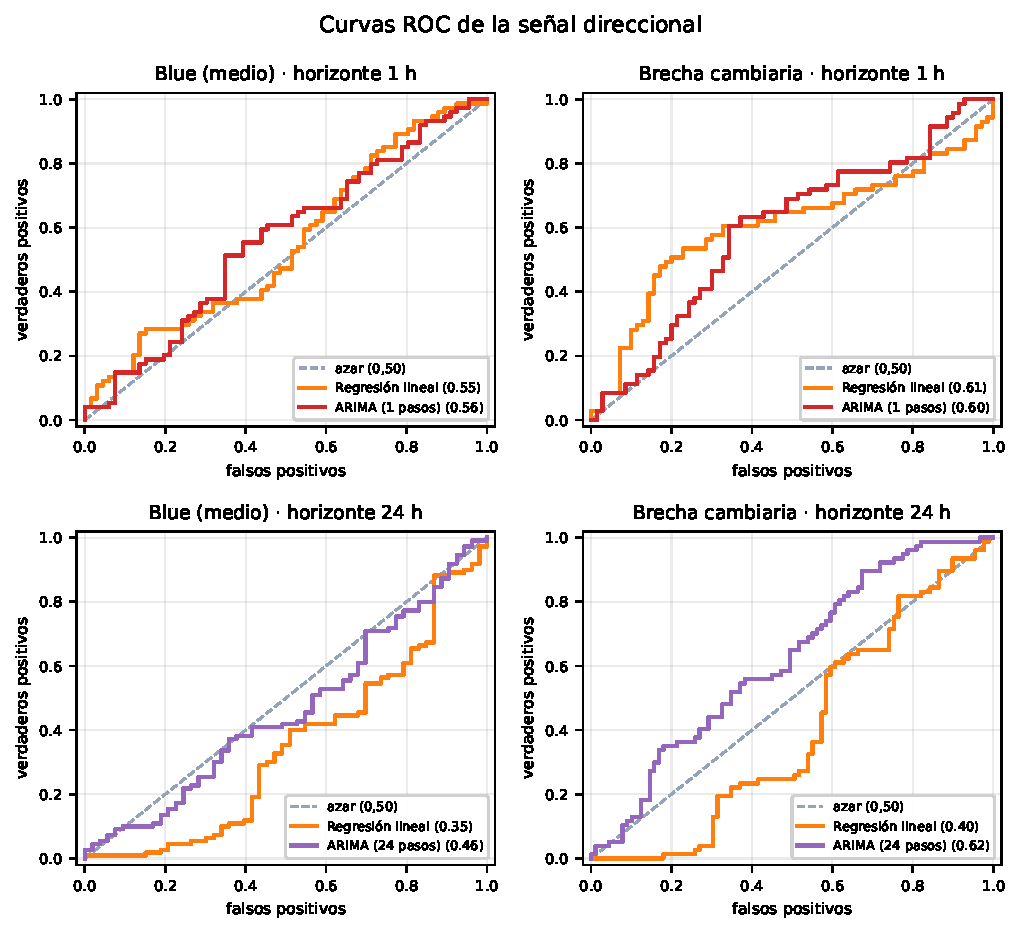
\includegraphics[width=\textwidth]{fig_roc.pdf}
\caption{Curvas ROC de la señal direccional, por horizonte (filas) y target
(columnas). La diagonal punteada es el azar (AUC $=0{,}50$). A una hora ninguna
curva pasa de $0{,}61$; a un día la brecha alcanza $0{,}62$ pero el nivel del
blue cae por debajo de $0{,}50$, y la regresión lineal queda en
$0{,}35$--$0{,}40$, peor que el azar.}
\label{fig:roc}
\end{figure}

\textbf{Lectura.} A una hora la discriminación es débil (AUC $0{,}55$--$0{,}61$),
coherente con un mercado casi impredecible. A un día la brecha mejora ($0{,}62$)
mientras el nivel cae bajo el azar, porque el sesgo de nivel de la regresión
invierte el signo de sus predicciones.

\subsection{Limitaciones de la evaluación}

\begin{itemize}
  \item El ahorro supone fijar el precio con el pronóstico; a precio de mercado
        es cero.
  \item $C_{FP}$ y $C_{FN}$ no se estimaron con datos de la empresa: el
        resultado es un umbral de decisión, no una cifra contable.
  \item Una sola semana de evaluación: los umbrales deben revisarse con más
        ventanas antes de usarse operativamente.
\end{itemize}


% ------------------- WIP: fases 5--6 de CRISP-DM -------------------
% % ============================================================================
% WIP — Conclusiones. NO incluidas en el informe todavía (enfoque actual:
% fases 1--3 de CRISP-DM). Reactivar en main.tex cuando se cierre la evaluación.
% ============================================================================
\section{Conclusiones}
\label{sec:conclusiones}

\begin{itemize}
  \item Se construyó un pipeline reproducible de recolección y normalización
        con resultados tipados y trazabilidad por corrida
        (\texttt{data/manifest.json}), cubriendo las dos fuentes del proyecto: la API
        dolarbluebolivia.click y la Gaceta Oficial \cite{dolarblue2026api}.
  \item Se dejó preparada (fases 1--3 de CRISP-DM) la base para predecir el
        nivel del paralelo y la brecha a horizontes de 1--7 días, con
        partición temporal y línea base naïve \cite{hyndman2021forecasting}.
  \item Este informe es, a su vez, parte del entregable: se regenera
        íntegramente (figuras, tablas, diagramas y PDF) con un único comando
        (comando en el Apéndice) desde los últimos CSV disponibles.
\end{itemize}

\subsection{Trabajo futuro}

\begin{itemize}
  \item Modelar y evaluar la previsión (Objetivo 1) y la relación entre la
        Gaceta y la brecha (Objetivo 2) con validación walk-forward
        \cite{box2015timeseries}.
  \item Respetar la cuota semanal de la API ($\sim$30 llamadas por corrida):
        ingestas programadas, no exploratorias.
\end{itemize}
  % Conclusiones (tras evaluación)

\footnotesize
\bibliography{refs}

\end{document}
